\documentclass{template_svk}

\usepackage[utf8]{inputenc}
%\usepackage[czech]{babel}
\usepackage{url}

\def\mtt#1{{\footnotesize\tt#1}}
\def\comm#1{\mtt{\char92#1}}

\begin{document}

\title{ARMv6 Processor Emulator for\\Raspberry Pi Environment Emulation}

% Autoři
 \author{Jakub Šilhavý}{student of the master
   degree program Applied Sciences, field of study Software Engineering,\\e-mail: silhavyj@students.zcu.cz}

\maketitle

\section{Introduction}

ARM stands out as one of the most widely embraced  computer architectures, finding application across a diverse range of domains. Its utility extends from low-power solutions and affordable microcontrollers to real-time applications and safety-critical systems, encompassing fields such as medical devices, the automotive industry, and aviation. Furthermore, ARM plays a significant role in personal computers and the cell phone industry, currently powering more than 99\% of the world's smartphones (\cite{ARM-history}).

Emulating such an extensively adopted architecture can assist in illustrating concepts of computer organization and operating systems. Additionally, it offers advantages in the field of software development, particularly when immediate access to a development board may not be feasible. Furthermore, it provides a layer of abstraction, allowing developers to experiment with potentially risky code without the concern of damaging real hardware.


\section{Existing Solutions}

Several available solutions, such as QEMU, CPUlator, and ARMSim\#, can be employed for emulating the ARM architecture. However, as the thesis concludes, their emulation capabilities may be limited, as most of them lack some of the more advanced system-related features, such as the ability to switch CPU modes or implement paging, which is indispensable in operating system development. Consequently, the thesis aimed to develop an extensible Raspberry Pi Zero emulator capable of emulating KIV-RTOS, an educational real-time operating system developed at the University of West Bohemia (\cite{KIV-RTOS}).

\section{Proposed Solution - ZeroMate}

ZeroMate was developed to address the challenges associated with the existing solutions. It was meticulously designed in a modular fashion, enabling users to seamlessly connect custom third-party peripherals such as displays, sensors, and actuators. These peripherals can be developed independently of the core system, providing users with flexibility and customization options. It was created with the aim of giving users a comprehensive visual overview of the entire system, allowing them to examine the current contents of various core components, such the CPU registers and RAM.

\newpage

Furthermore, it offers insights into the current configurations of various BCM2835 peripherals, including the GPIO pins, interrupt controller, ARM timer, MiniUART, BSC (I2C), and more. Moreover, it boasts support for fundamental debugging features, thereby simplifying the debugging process for cross-compiled applications. Additionally, the emulator incorporates coprocessor support, empowering users to harness features like floating-point numbers or virtual addressing.

\begin{figure}[!ht]
	\centering
	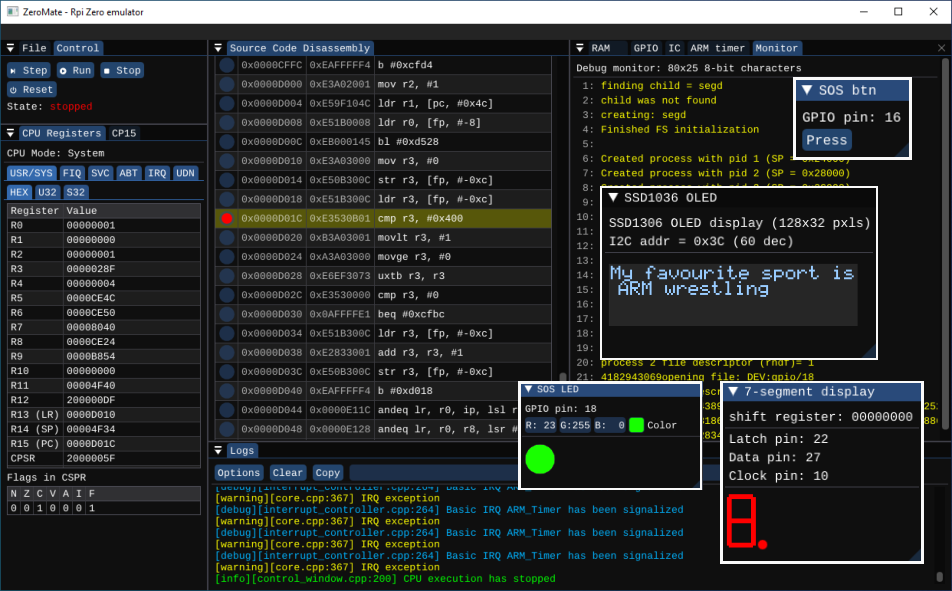
\includegraphics[width=0.8\textwidth]{img/screenshot.pdf}
	\caption{ZeroMate’s graphical user interface}
\end{figure}

\section{Conclusion}

The core of the emulator underwent rigorous testing through an extensive set of unit tests, addressing its fundamental yet crucial functionalities that other parts of the system heavily depend on. Unit tests cover approximately 78\% of the core’s functionality. Functional testing integrated different components of the emulator working alongside to execute specific tasks, such as blinking an LED using a timer interrupt or scheduling processes running in userspace. The final phase of testing, system testing, was conducted by students enrolled in the KIV/OS class to assess its overall usability in practice. Using KIV-RTOS, ZeroMate’s average speed of emulation was measured to be 4.84 mega instructions per second \footnote{The experiment was conducted on the Lenovo ThinkPad P50 laptop, running the Windows 10 operating system. The laptop is equipped with an Intel(R) Core(TM) i7-6820HQ CPU running at 2.70GHz and 16GB of RAM. In terms of \texttt{C++}, the \texttt{std::chrono::high\_resolution\_clock} class was employed for measuring execution speed in nanoseconds.}.

\begin{thebibliography}{99}\itemsep=.75ex%
	
	\bibitem[Arm Editorial Team (2023)]{ARM-history}
	Arm Editorial Team. (2023). \textit{The Official History of Arm}.
	Available from: \url{https://newsroom.arm.com/arm-official-history}
	[Accessed 25th September 2023].
	
	\bibitem[Martin Úbl (2021)]{KIV-RTOS}
	Martin Úbl (2021). \textit{KIV-RTOS - An educational operating system for bare-metal Raspberry Pi Zero W (BCM2835-based board)}. Available from: \url{https://github.com/MartinUbl/KIV-RTOS} [Accessed 27th September 2023].

	
\end{thebibliography}


\end{document}
